\chapter{Experimentos}

\section{Controlador pequeños ángulos}
\begin{figure}[htb!]
	\centering
	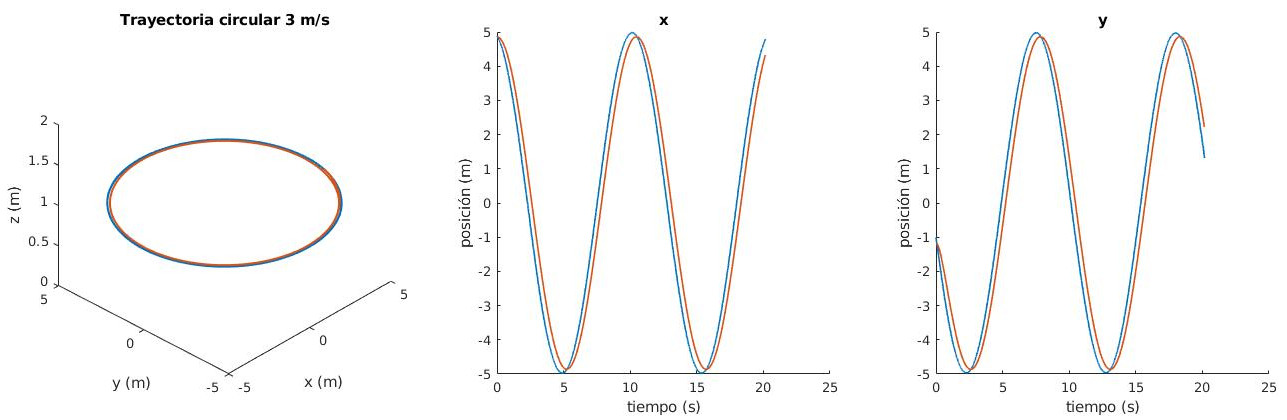
\includegraphics[width=\textwidth]{imagenes/circle3ms}
	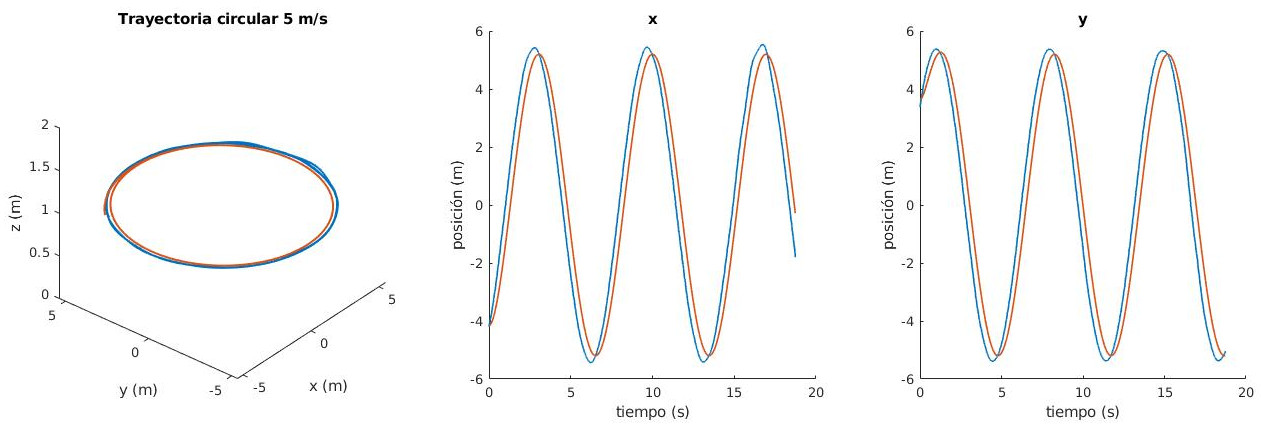
\includegraphics[width=\textwidth]{imagenes/circle5ms}
	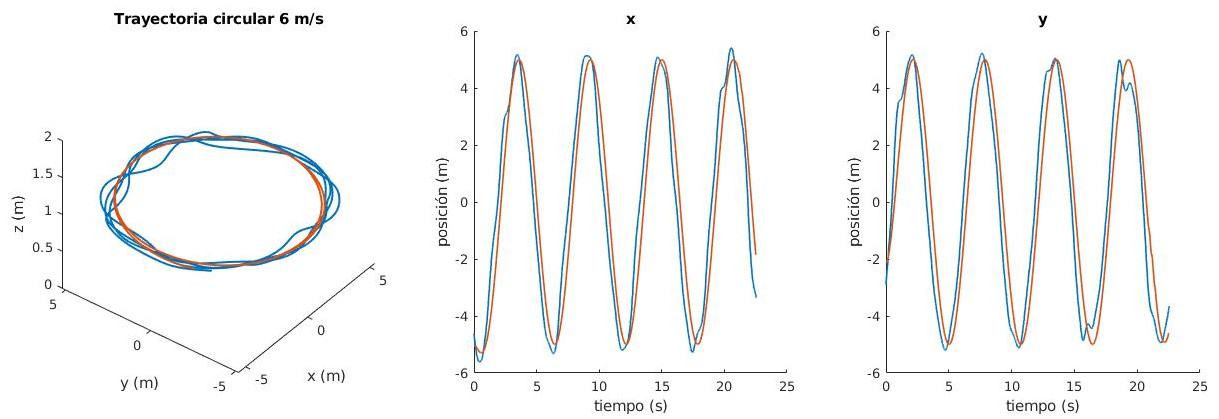
\includegraphics[width=\textwidth]{imagenes/circle6ms}
	\caption{Trayectorias circulares a 3, 5 y 6 m/s empleando un controlador para angulos pequeños}
	\label{circle:slow}
\end{figure}
\section{Controlador grandes  ángulos}

\begin{figure}[htb!]
	\centering
	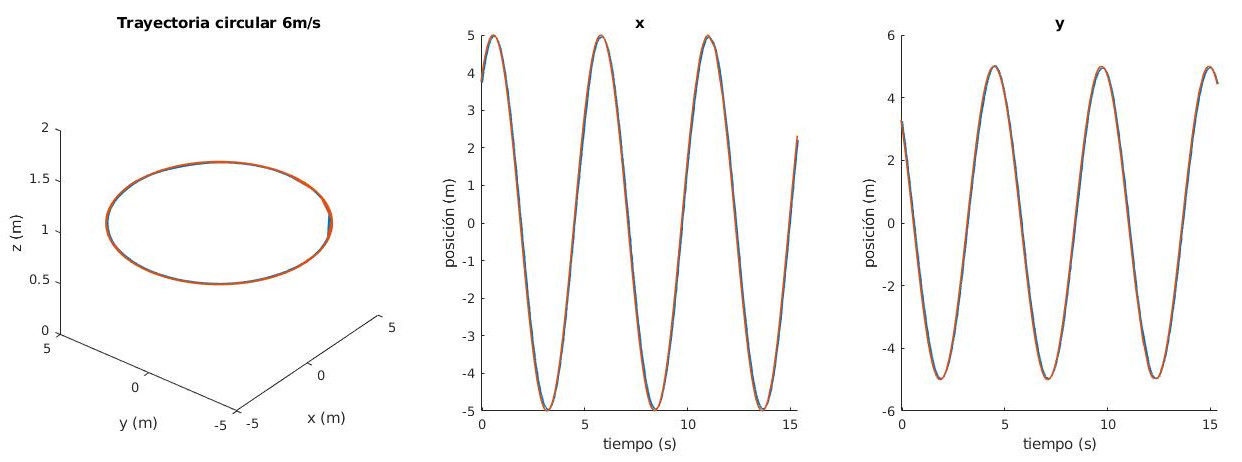
\includegraphics[width=\textwidth]{imagenes/fast_circle6ms}
	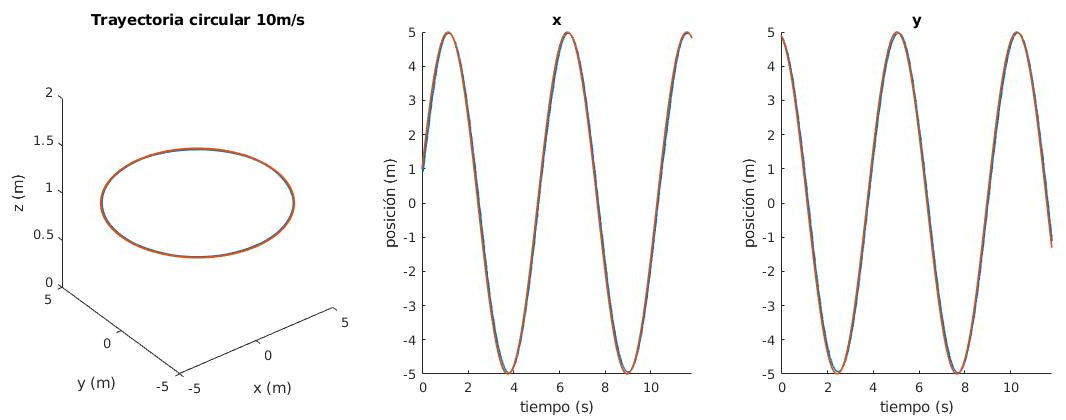
\includegraphics[width=\textwidth]{imagenes/fast_circle10ms}
	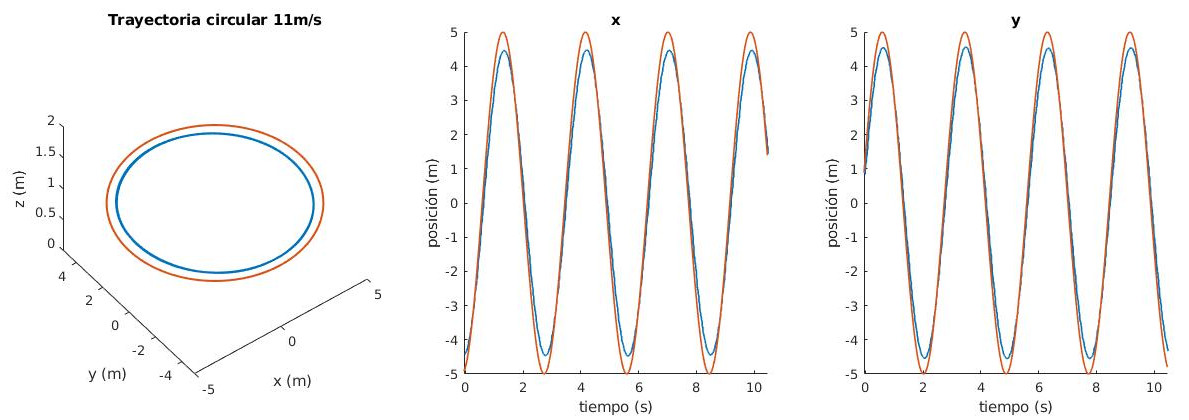
\includegraphics[width=\textwidth]{imagenes/fast_circle11ms}
	\caption{Trayectorias circulares a 6, 10 y 11 m/s empleando un controlador para angulos grandes}
	\label{circle:fast}
\end{figure}

\section{Circuito completo}
\subsection{\tb{Normal speed}}

\begin{figure}[htb!]
	\centering
	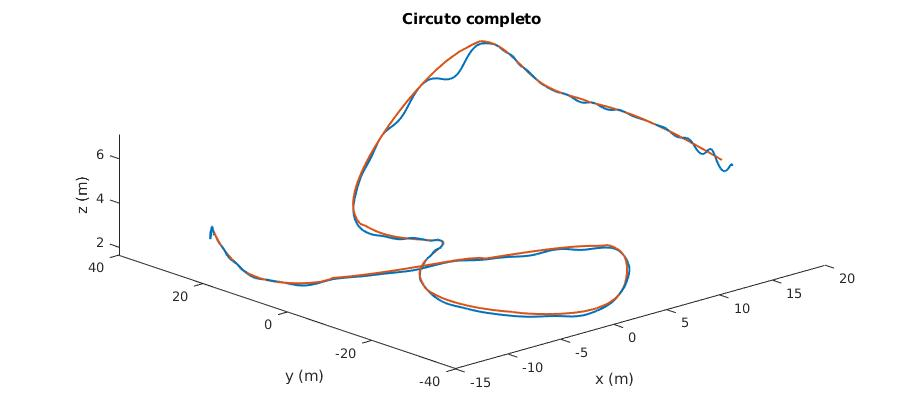
\includegraphics[width=\textwidth]{imagenes/circuitFigure}
	\caption{}
	\label{exp1:1}
\end{figure}

\begin{figure}[htb!]
	\centering
	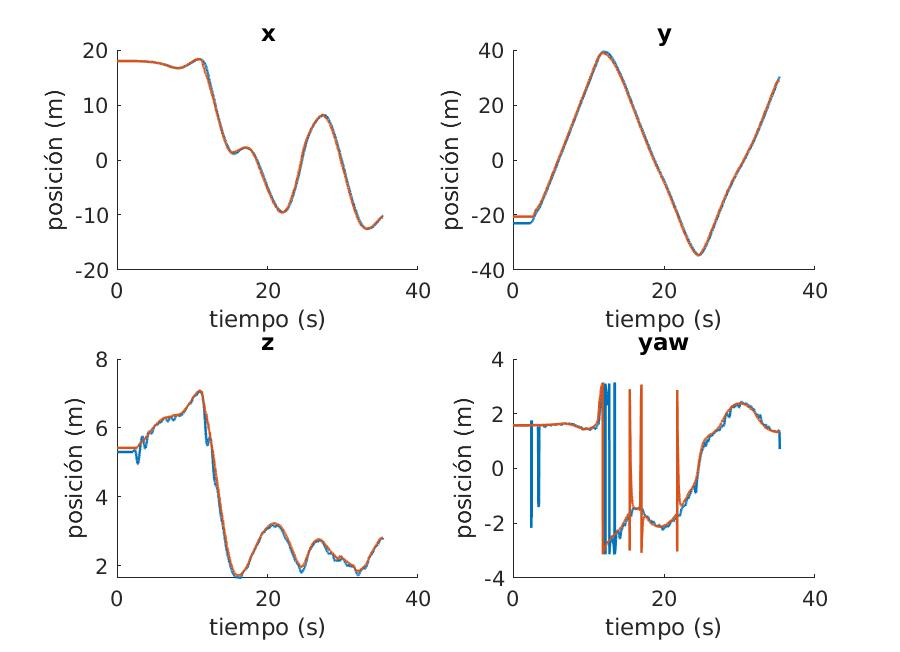
\includegraphics[width=\textwidth]{imagenes/positionFigure}
	\caption{}
	\label{exp1:2}
\end{figure}

\begin{figure}[htb!]
	\centering
	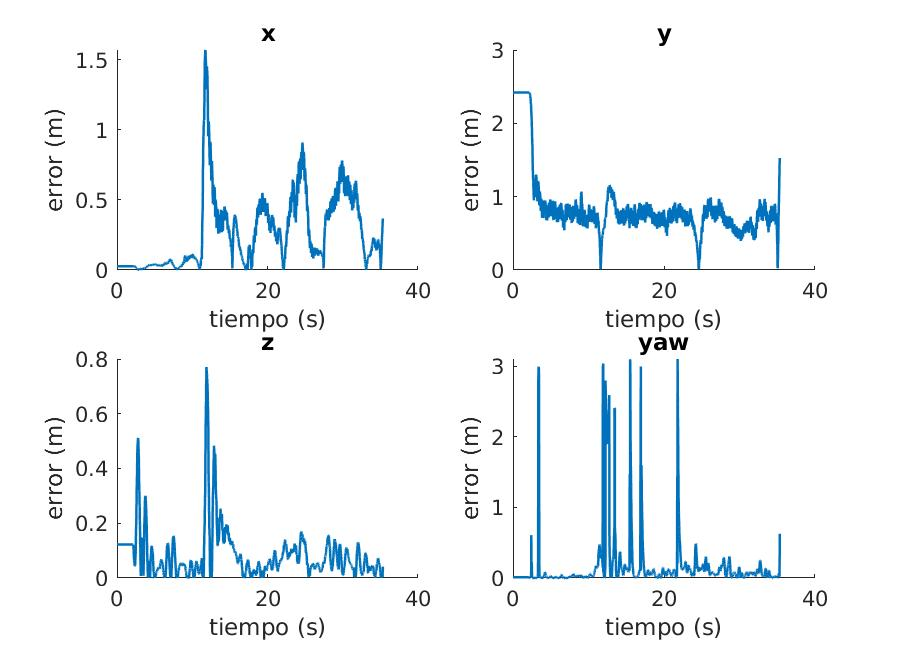
\includegraphics[width=\textwidth]{imagenes/errorFigure}
	\caption{}
	\label{exp1:3}
\end{figure}



\begin{table}[htb!]
	\centering
	
	\begin{tabular}{l|c|c|c|}
		$\empty$&Eje x&Eje y&Eje z\\
		\midrule
		Error máximo (m)&1.5685&1.1577&0.7707\\
		Error medio (m) &0.3143&0.7306&0.0796\\
		
	\end{tabular}
	\caption{Errores de seguimiento durante el recorrido del circuito.}
\end{table}


\begin{table}[htb!]
	\centering
	\begin{tabular}{l|c|c|}
		$\empty$&Máxima& Media\\
		\midrule
		Velocidad (m/s)&7.4199&5.8565\\
		
	\end{tabular}
	\caption{Velocidad del cuadricóptero durante el recorrido del circuito.}
\end{table}


\subsection{\tb{BESTspeed}}

\begin{figure}[htb!]
	\centering
	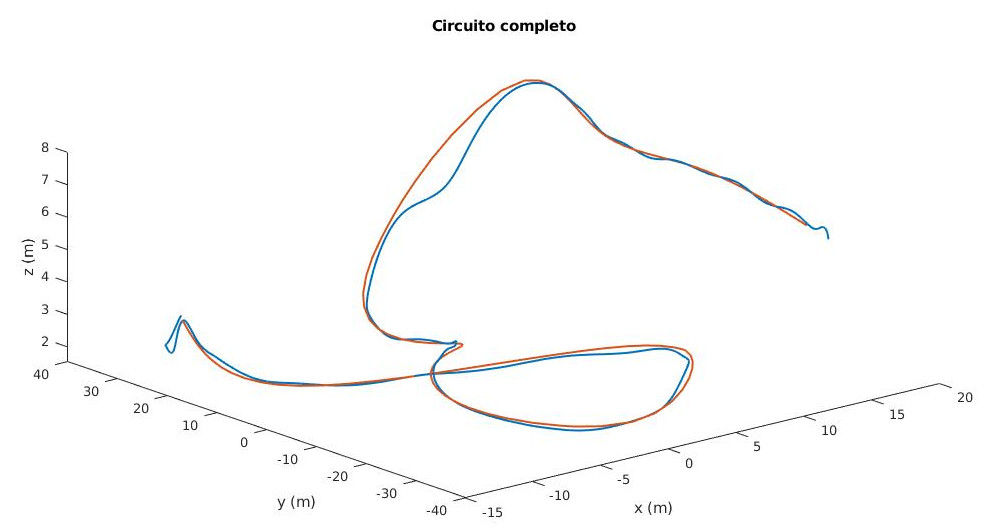
\includegraphics[width=\textwidth]{imagenes/best_circuitFigure}
	\caption{}
	\label{exp1:1}
\end{figure}

\begin{figure}[htb!]
	\centering
	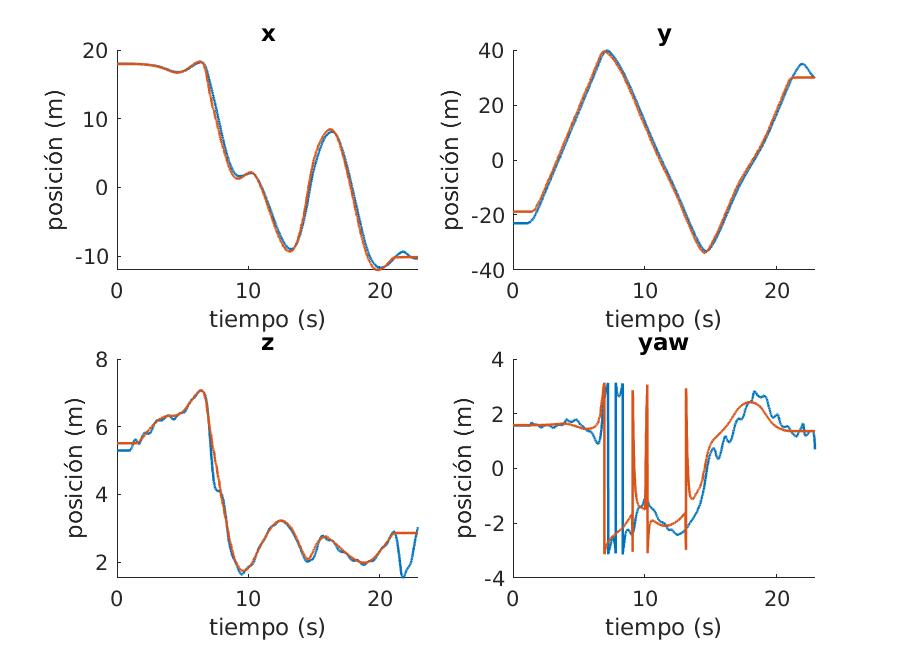
\includegraphics[width=\textwidth]{imagenes/best_positionFigure}
	\caption{}
	\label{exp1:2}
\end{figure}

\begin{figure}[htb!]
	\centering
	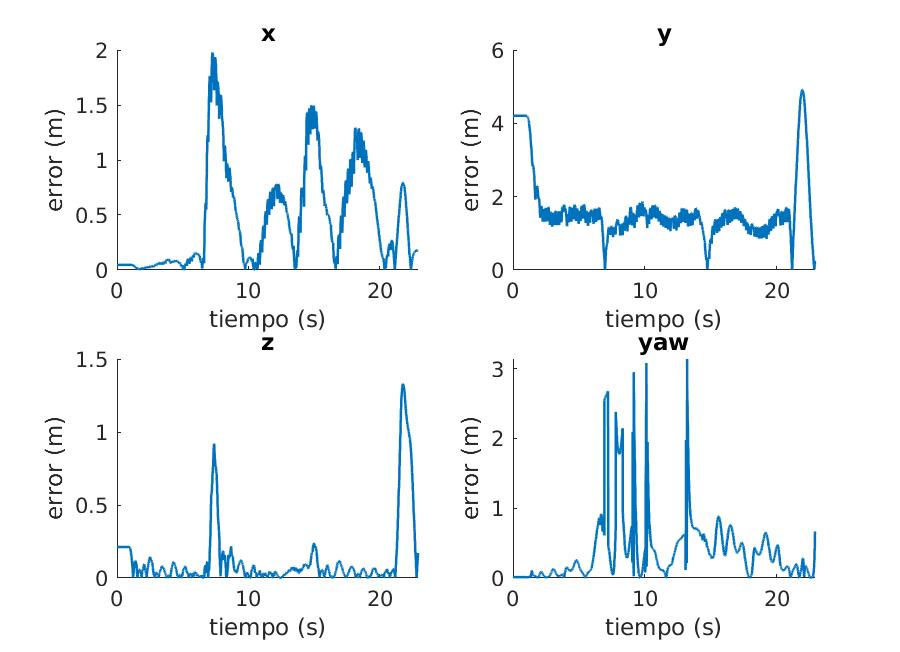
\includegraphics[width=\textwidth]{imagenes/best_errorFigure}
	\caption{}
	\label{exp1:3}
\end{figure}



\begin{table}[htb!]
	\centering
	\begin{tabular}{l|c|c|c|}
		$\empty$&Eje x&Eje y&Eje z\\
		\midrule
		Error máximo (m)&1.9776&1.9181&1.3302\\
		Error medio (m) &0.5973&1.4826&1.1413\\
		
	\end{tabular}
	\caption{Errores de seguimiento durante el recorrido del circuito.}
\end{table}



\begin{table}[htb!]
	\centering
	\begin{tabular}{l|c|c|}
		$\empty$&Máxima& Media\\
		\midrule
		Velocidad (m/s)&10.4948&9.3936\\
		
	\end{tabular}
	\caption{Velocidad del cuadricóptero durante el recorrido del circuito.}
\end{table}






\section{Experimentos en simulación}
\section{Experimentos en real}